\chapter{Fuzzy Control System} \label{ch:fcs}

Fuzzy logics provide a way of quantitatively interpreting and calculating attributes or reasonings described by vague languages. In contrast to classical control methods where variables are numbered precisely and control laws described clearly by mathematical equations, a fuzzy controller uses objective terms such as ``good'', ``bad'', ``high'', ``low'', ``very'', ``a little'' to describe variables, and use rules ``if something then something'' to determine the control signals. This makes a fuzzy controller naturally good at realizing human knowledge base into practice.

Different from ANN which is highly data driven and requires a lot of samples and computations to train a network, a fuzzy controller is an expert-based system that requires only the membership functions used for fuzzification of variables and a set of rules for inference. ANN may reveal the building bricks of a human brain, while fuzzy control system reflects how a human interprets the knowledge that he learns from past experience and uses in his daily life. This feature of a fuzzy control system is a bless and a curse at the same time. Fuzzy control system does not rely on training, thus is handy when there are few training samples. On the other hand, this also means that it cannot benefit from the accumulation of the samples and it is lack of evolving capability comparing with ANN and other evolutionary algorithms.

\section{Fuzzy Set and Fuzzy Relation}

Fuzzy set is not a set from mathematical perspective, but a projection derived from a set. Fuzzy set and fuzzy relation are the fundamentals of fuzzy logics. Details are given in the remaining of this section.

\subsection{Fuzzy Set}

The fundamentals of fuzzy logics and fuzzy control systems are built on fuzzy set and membership function. Fuzzy set is not a set from mathematical perspective, but a projection from a set to a real number between $[0, 1]$. The function used in the projection is called the member function of the fuzzy set.

Consider set $U$ with finite or infinite cardinality. Define a projection $\mu_{\utilde{A}}$ from $x \in U$ to $[0, 1]$ as follows.
\begin{eqnarray}
	\mu_{\utilde{A}} &:& x \in U \rightarrow [0, 1] \nonumber
\end{eqnarray}
This projection, together with its domain (also known as the universe of a fuzzy set) defines a fuzzy set. The projection $\mu_{\utilde{A}}$ is called the membership function of the fuzzy set $\utilde{A}$. The value of $\mu_{\utilde{A}}(x)$ for $x \in U$ describes in what extent $x$ belongs to $\utilde{A}$.

It is clear from the definition the difference between a set and a fuzzy set. For a set, an element either belongs to the set or does not belong to the set, which can be described by
\begin{eqnarray}
	\mu_{A}(x) = \left\{\begin{array}{cc}
		1 & x \in A \\
		0 & x \notin A
	\end{array}\right. \nonumber
\end{eqnarray}
where $\mu_{A}$ is a binary function. In contrast, fuzzy set defines a continuous functions $\mu_{\utilde{A}}$ which can take any value between $[0,1]$. From this stand, a fuzzy set is an extension to a set.

An example of a fuzzy set is given below. Let $U\geq 0$ be the age of a person. Define 2 fuzzy sets, ``young adult'' as $\utilde{A}$ and ``middle-aged adult'' as $\utilde{B}$, with membership function defined in Fig. \ref{ch:fcs:fig:fuzzysetexp}.

\begin{figure}
	\centering
	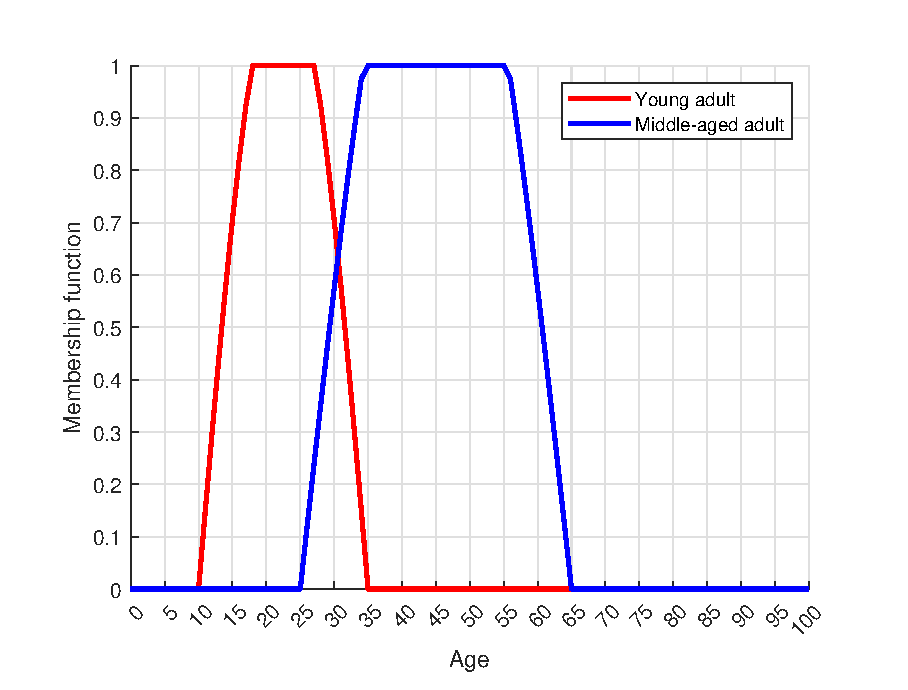
\includegraphics[width=250pt]{chapters/ch-fuzzy-control-system/figures/fuzzysetexp.eps}
	\caption{Membership function of fuzzy sets ``young adult'' and ``middle-aged adult''.} \label{ch:fcs:fig:fuzzysetexp}
\end{figure}

From Fig. \ref{ch:fcs:fig:fuzzysetexp}, we can see how a person is categorized according to the age. For example, a 5-year-old child is by no means a young adult or an adult, as $\mu_{A}=\mu_{B}(5)=0$ from the figure. A 27-year-old can be considered ``quite'' a young adult, with $\mu_{A}=0.8$, and ``somehow'' adult, with $\mu_{A}=0.3$.

The maximum value of a membership function is defined as the height of the fuzzy set. In many occasions the height is $1$, but it is not always the case. An element whose associated membership function equals to half of the height is called the crossover point.

It is possible to set up a threshold for the membership function, and derive a set from a fuzzy set as follows.
\begin{eqnarray}
	\utilde{A}_\alpha &=& \left\{x \middle| \mu_{\utilde{A}} (e) \geq \alpha \right\} \nonumber
\end{eqnarray}
Notice that $\utilde{A}_\alpha$ is a set (not a fuzzy set) known as the cut set of $\utilde{A}$. A fuzzy set can have infinite number of cut sets by choosing different $\alpha$. A fuzzy set can be derived from all its cut sets as follows.
\begin{eqnarray}
	\utilde{A} &=& \bigcup_{\alpha \in [0, 1]} \alpha A_\alpha \nonumber
\end{eqnarray}
where $\alpha A_\alpha$ is a fuzzy set defined on $A_\alpha$ with, universe $A_\alpha$ and membership function value $\alpha$. The $\cup$ calculates the union of fuzzy sets, more of which is introduced later.

Define the support and core of a fuzzy set as follows, respectively.
\begin{eqnarray}
	\textup{supp}(\utilde{A}) &=& \left\{x \middle| \mu_{\utilde{A}}(x) > 0 \right\} \nonumber \\
	C(\utilde{A}) &=& \left\{x \middle| \mu_{\utilde{A}}(x) = 1 \right\} \nonumber
\end{eqnarray}

A fuzzy set $\utilde{A}$ can be represented by its base set $A$ together with associated membership functions $\mu_{\utilde{A}}$. Alternatively, use the following
\begin{eqnarray}
	\utilde{A} &=& \sum_{i} \dfrac{\mu_{\utilde{A}}(x_i)}{x_i} \nonumber \\
	\utilde{A} &=& \int_{E} \dfrac{\mu_{\utilde{A}}(x)}{x} \nonumber
\end{eqnarray}
to represent a fuzzy set with discrete and continuous universe, respectively. Notice that in the above representation, ``$/$'', ``$\sum$'', and ``$\int$'' are not division, summation and integration, but just conventional notations used in the fuzzy set theory.

\subsection{Fuzzy Set Operations}

Operations such as union and intersection are defined on fuzzy sets. They are summarized in Table \ref{ch:fcs:tab:fuzzysetoperation}.

\begin{table}[h]
	\centering
	\begin{tabular}{lll}
		\hline
		Operation & Symbol & Membership Function \\
		\hline
		Union & $\utilde{A} \cup \utilde{B}$ & $\mu_{\utilde{A} \cup \utilde{B}}(e) = \max(\mu_{\utilde{A}}(e), \mu_{\utilde{B}}(e))$ \\
		Intersection & $\utilde{A} \cap \utilde{B}$ & $\mu_{\utilde{A} \cap \utilde{B}}(e) = \min(\mu_{\utilde{A}}(e), \mu_{\utilde{B}}(e))$ \\
		Complement & $\utilde{A}'$ & $\mu_{\utilde{A}'}(e) = 1 - \mu_{\utilde{A}}(e)$ \\
		\hline
	\end{tabular}
	\caption{Commonly used fuzzy set operations.}
	\label{ch:fcs:tab:fuzzysetoperation}
\end{table}

Notice that Table \ref{ch:fcs:tab:fuzzysetoperation} gives only one out of many ways to define these operations. There are other ways to define them. For example, for complement, there is Sugeno's complement and Yager's complement as follows. The ones given in Table \ref{ch:fcs:tab:fuzzysetoperation} is the most commonly used definition.
\begin{eqnarray}
	N_s(e) &=& \dfrac{1-e}{1+\lambda e} \nonumber \\
	N_w(e) &=& (1-a^w)^{\frac{1}{w}} \nonumber
\end{eqnarray}

More operations can be found in \cite{mizumoto1981fuzzy}.

\subsection{Commonly Used Membership Functions}

Membership functions can be chosen flexibly as long as it is bounded by $[0, 1]$ for each element. There are some commonly used ones that has been proved useful in general problems as shown in Fig. \ref{ch:fcs:fig:commonmf}. They, together with their combinations, are widely used in fuzzy control system design.

\begin{figure}
	\centering
	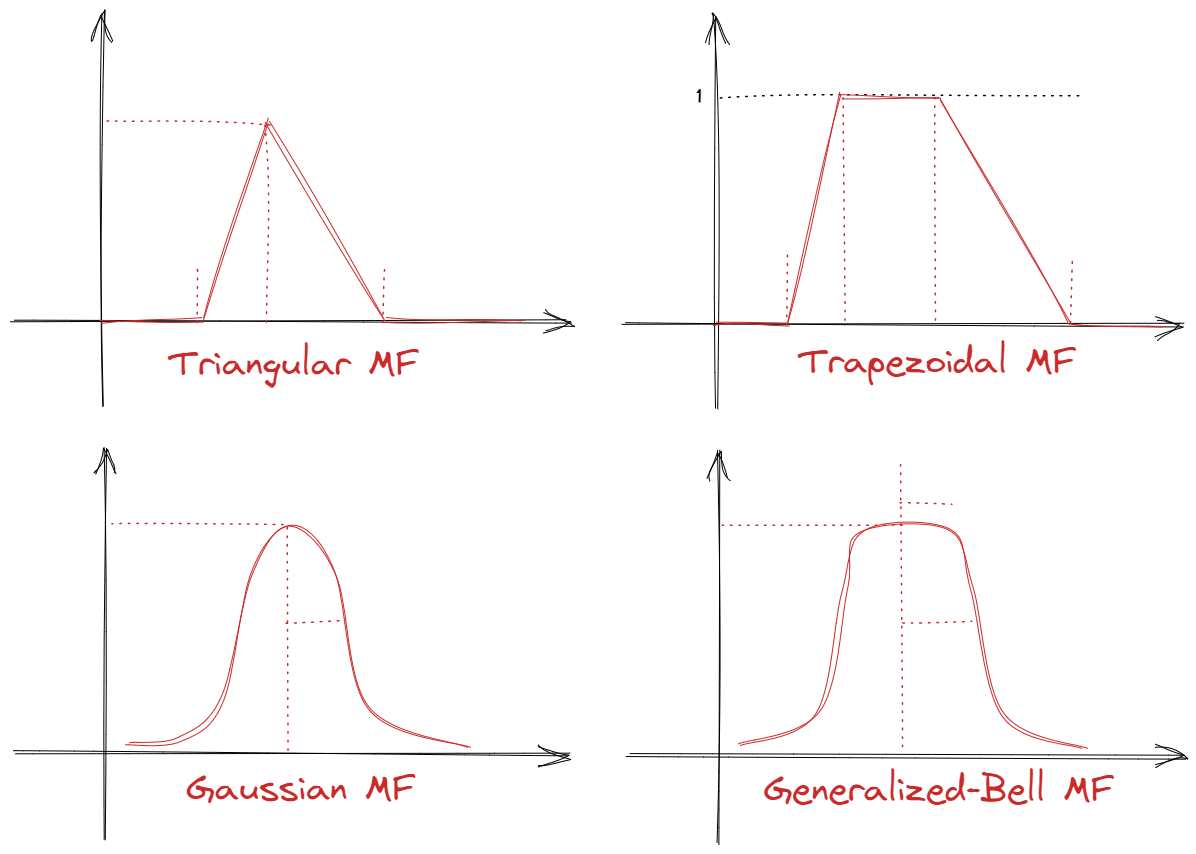
\includegraphics[width=350pt]{chapters/ch-fuzzy-control-system/figures/commonmf.png}
	\caption{Commonly used membership functions.} \label{ch:fcs:fig:commonmf}
\end{figure}

MATLAB provides built-in functions to generate the functions in \ref{ch:fcs:fig:commonmf}, such as \verb|trimf| for triangular membership function, \verb|trapmf| for trapezoidal function, \verb|gaussmf| for Gaussian, and \verb|gbellmf| for generalized-bell function, respectively. There are other membership functions built-in to MATLAB as well.

\subsection{Fuzzy Relation}

In set theory, a relation of two elements is defined using sets. For example, let $a, b \in \mathbb{R}$. Let a customized relation ``$\oplus$'' be defined on $\mathbb{R} \times \mathbb{R} = \mathbb{R}^2$. We can say $a \oplus b$ if and only if there is a set defined on $\mathbb{R}^2$ associated with ``$\oplus$'' relation, and $(a,b)$ is in that set. Here ``$\times$'' denotes the Cartesian product.

Fuzzy relation is defined likewise, except that the set is replaced with fuzzy set as follows. Let $u\in U$, $v \in V$ be two variables with the same or different domains, and $D=U \times V$. The fuzzy relation of ``$\oplus$'' of two elements $u$ and $v$ is defined by the following fuzzy set
\begin{eqnarray}
	\mu_{\utilde{D}} (u,v) &\in& [0, 1] \nonumber
\end{eqnarray}
associated with ``$\oplus$''.

It is possible to use a matrix to record the fuzzy relations, in which case the matrix is called a fuzzy matrix as it is made up of membership functions. Other choice include fuzzy graph, which takes advantage of graph theory to represent the fuzzy relation of different nodes in a universe.

The relation can be derived from chains. For example, consider relation $P$ defined one $X \times Y$, and $Q$ on $Y \times Z$. A relation on $X, Z$ can be derived. One way (this is not the only way) is to use
\begin{eqnarray}
	\mu_{X \times Z}(x, z) &=& \sup \left[\min\left(\mu_{X\times Y}(x, y), \mu_{Y\times Z} (y, z)\right)\right] \nonumber
\end{eqnarray}

\section{Fuzzy Control System}

Fuzzy control system is a practice of utilizing fuzzy logics in engineering. It mainly includes fuzzification of the physical measurement signals to fuzzy variables, fuzzy inference, and defuzzification of the fuzzy variables to physical control signals. Membership functions are used in the fuzzification and defuzzification of signals, and rules are used in the fuzzy inference.

A simple schema of a fuzzy control system is given in Fig. \ref{ch:fcs:fig:fuzzyschemasimple}. Details are covered in the remaining of this section.

\begin{figure}
	\centering
	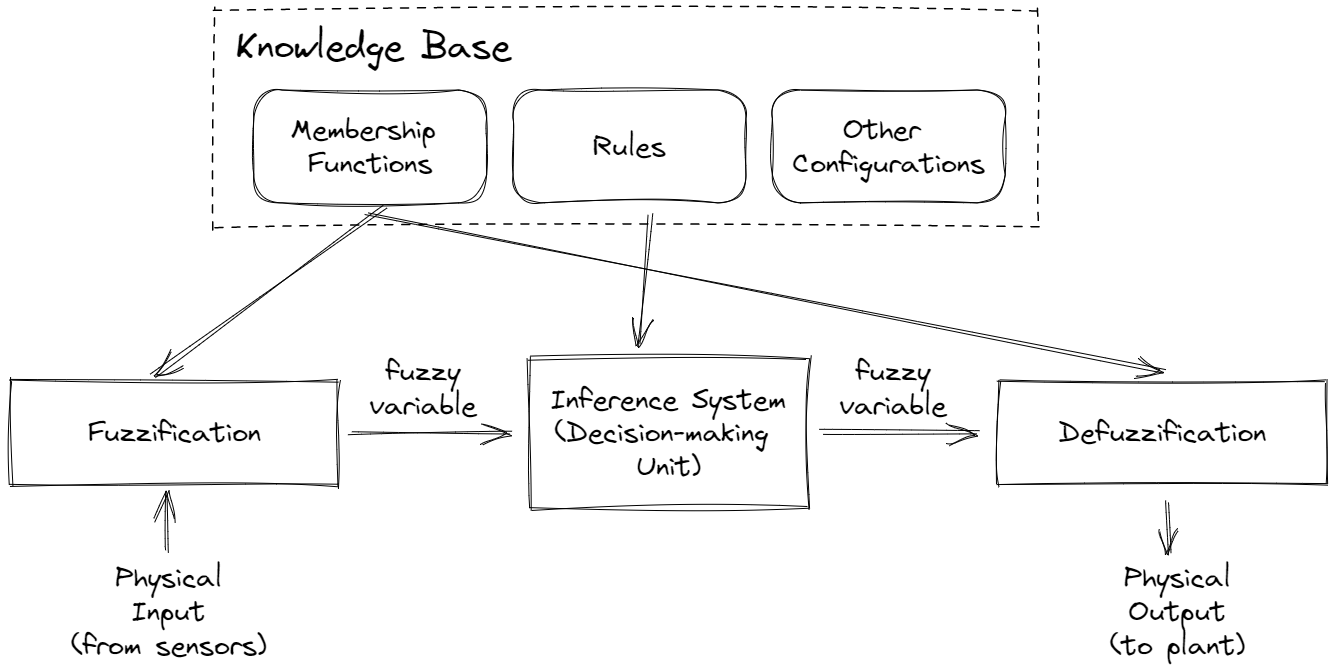
\includegraphics[width=350pt]{chapters/ch-fuzzy-control-system/figures/fuzzyschemasimple.png}
	\caption{A simple schema for a fuzzy control system.}
	\label{ch:fcs:fig:fuzzyschemasimple}
\end{figure}

\subsection{Fuzzification}

xxx

\subsection{Fuzzy Interface}

xxx

\subsection{Fuzzy Controller Design}

xxx

\subsection{Fuzzy Controller Performance Analysis}

xxx

\section{Fuzzy Modeling and Fuzzy System Identification}

xxx

\section{Fuzzy System Auto-tuning}

The performance of a fuzzy control system is mainly determined by the choice of membership functions, inference rules and defuzzification methods. In the case where there is no such an expert that can carefully design everything, a data-driven approach can be implemented that automatically tunes the parameters setup in a fuzzy control system for the optimal performance. 

Notice that the auto-tuning does not change the fact that a fuzzy control system is a rule-based expert system. Therefore, the advantage of fuzzy system being intuitive to interpret persists.

Nowadays, the most popular data-driven approach for data analysis is artificial neural network. It is possible to use ANN to find the optimal parameters of a fuzzy system, hence, fuzzy neural networks. 















\section{Fuzzy Control System Design Using MATLAB}

MATLAB fuzzy logic toolbox provides tools to define membership functions and fuzzy inference systems. They are introduced in this section via examples.

\subsection{Example: Vibration Detection}

Consider the example given below. Design and implement the system in MATLAB as follows.

\begin{shortbox}
\Boxhead{Vibration Detection from Measurement Signal}

Oscillation has been detected from a continuously sampled signal. The oscillation might be caused by system process dynamics, system vibration, or measurement noise. The oscillation frequency and amplitude together help to reveal the cause of the oscillation, specifically the likelihood that the oscillation is caused by system vibration.

The input to the system is the oscillating measurement signal sampled at $1Hz$. An FFT is applied to the signal to get the oscillation frequency and amplitude, which lay in the range of $[0, 0.5] (Hz)$ and $[0, 10]$, respectively. The oscillation frequency and amplitude is then sent to the fuzzy controller.

In the fuzzy controller, the two signals are fuzzifized to form fuzzy variables. The fuzzy variables are passed to the fuzzy inference system, where rules are defined to determine the likelihood that the oscillation is caused by vibration, which is also a fuzzy variable. Finally, the likelihood fuzzy variable is defuzzifized to obtain the vibration likelihood, which should be a variable in $[0,1]$.

\end{shortbox}

\vspace{0.1in}
\noindent \textbf{Membership Functions for Input and Outputs}
\vspace{0.1in}

The first step in solving this problem is to understand how an human expert would interpret oscillation frequency and amplitude, and derive the likelihood from them. Take oscillation frequency as an example. It is agreed on that a frequency that is too low or too high may indicate something other than vibration. For example, frequency lower than $0.05Hz$ will be categorized as ``low''. Similarly, frequency higher than $0.4Hz$ is probably too ``high'' for vibration. Frequency around $0.2Hz$ is the ``fine'' frequency, which increases the likelihood of vibration.

Imagine asking many experts on how they categorize each frequency $0.01Hz, 0.02Hz, ..., 0.5Hz$ into one of the 3 categories ``low'', ``fine'' or ``high''. Consider using the interview results to form the membership for the 3 categories as given in Fig. \ref{ch:fcs:fig:exp_vibration_detection_mf_freq}. The curves in Fig. \ref{ch:fcs:fig:exp_vibration_detection_mf_freq} is obtained by fitting the ``percentage of agreement'' using trapezoidal functions. Figure \ref{ch:fcs:fig:exp_vibration_detection_mf_freq} can be interpreted as in what extend one would agree that the specified frequency shall belong to a category.

\begin{figure}
	\centering
	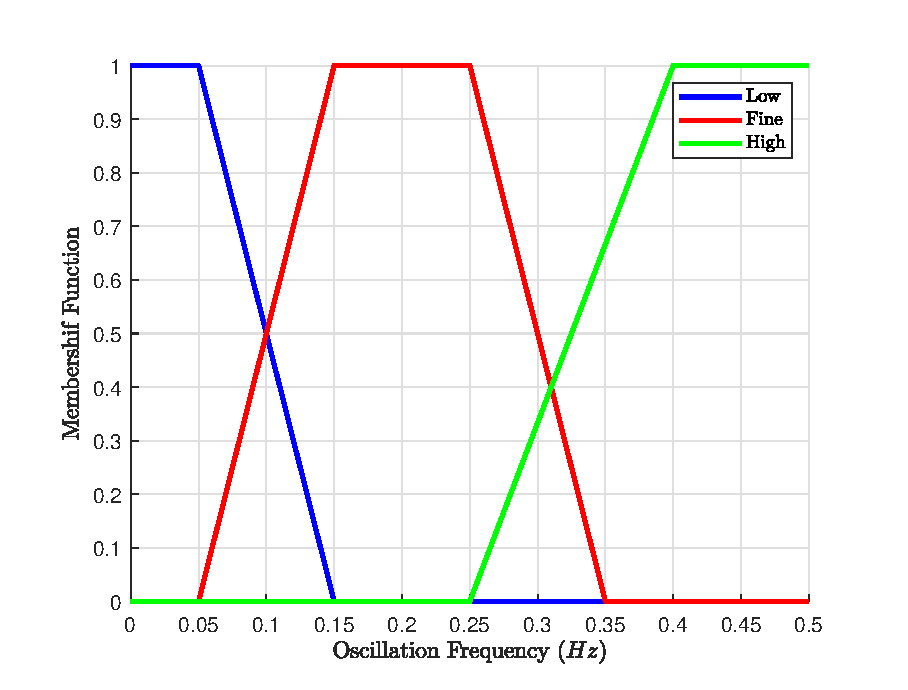
\includegraphics[width=250pt]{chapters/ch-fuzzy-control-system/figures/exp_vibration_detection_mf_freq.eps}
	\caption{Membership functions for 3 fuzzy sets ``low'', ``fine'' and ``high'' defined on input signal oscillation frequency.}
	\label{ch:fcs:fig:exp_vibration_detection_mf_freq}
\end{figure}

The same applies to the oscillation amplitude, where 2 categories are defined, namely ``low'' and ``fine'', as shown by Fig. \ref{ch:fcs:fig:exp_vibration_detection_mf_amp}. Instead of using trapezoidal functions, generalized bell functions are used to fit the interview results.

\begin{figure}
	\centering
	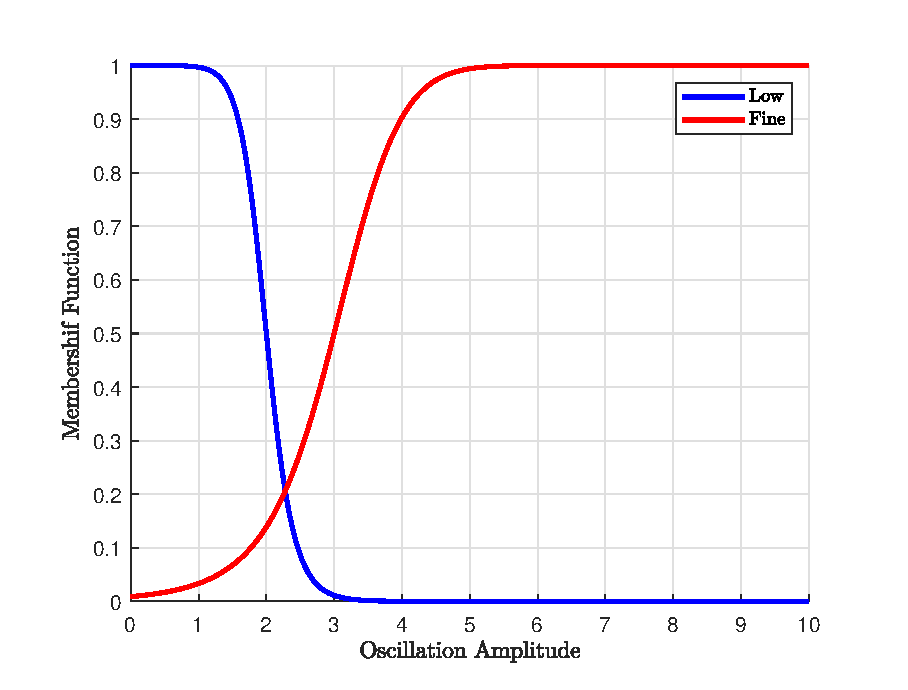
\includegraphics[width=250pt]{chapters/ch-fuzzy-control-system/figures/exp_vibration_detection_mf_amp.eps}
	\caption{Membership functions for 2 fuzzy sets ``low'' and ``fine'' defined on input signal oscillation amplitude.}
	\label{ch:fcs:fig:exp_vibration_detection_mf_amp}
\end{figure}

With the above defined membership functions, each frequency and amplitude can be translated into a fuzzy variable using fuzzification. For example, frequency $0.12Hz$ is $[0.3, 0.7, 0]$ where the three values in the vector represents the membership functions values of the given frequency mapping to each fuzzy set.

The output of the system is the likelihood of vibration of the system, scaled by a parameter in $[0, 1]$. Define 4 fuzzy sets, namely ``very likely'', ``likely'', ``unlikely'', ``very unlikely'', as shown in Fig. \ref{ch:fcs:fig:exp_vibration_detection_mf_likelihood}.

\begin{figure}
	\centering
	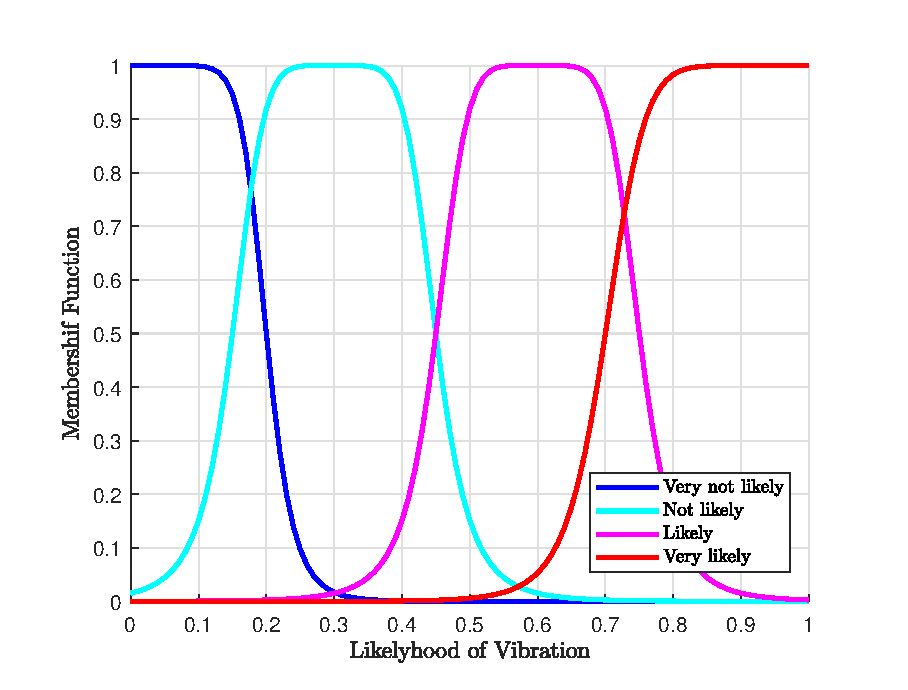
\includegraphics[width=250pt]{chapters/ch-fuzzy-control-system/figures/exp_vibration_detection_mf_likelihood.eps}
	\caption{Membership functions for 4 fuzzy sets ``very unlikely'', ``unlikely'', ``likely'' and ``very likely'', defined on input signal oscillation amplitude.}
	\label{ch:fcs:fig:exp_vibration_detection_mf_likelihood}
\end{figure}

With the above defined membership functions, each likelihood fuzzy variable can be translated into the likelihood of the occurrence of vibration via defuzzification. For example, likelihood fuzzy variable $[0, 0.1, 0.3, 0.9]$ means that the the likelihood is not at all ``very unlikely'', a tiny little bit ``unlikely'', somewhat ``likely'', and quite much ``very likely''. Intuitively, this should translate into a high likelihood around $0.7\sim 0.9$ using Fig. \ref{ch:fcs:fig:exp_vibration_detection_mf_likelihood}.

There are different ways of translating the output fuzzy variables into a physical signal, such as ``centroid'', ``bisector'', ``middle of maximum'', etc. More details can be found in MATLAB help document under ``defuzzification methods''. For example, $[0, 0.1, 0.3, 0.9]$ would translate into $0.73$ using membership function given in Fig. \ref{ch:fcs:fig:exp_vibration_detection_mf_likelihood} using centroid method, and $0.79$ if using bisector method instead.

\vspace{0.1in}
\noindent \textbf{Inference}
\vspace{0.1in}

Fuzzy inference system is rule-based. Examples of the rules may include the following. Notice that in this example, all combinations of oscillation frequency and amplitude are listed. This is not always necessary in practice. Some of the rules may seem conflict with each other. This does not matter as the fuzzy controller will balance the weight of each output fuzzy set.
\begin{itemize}
	\item If oscillation frequency is fine and oscillation amplitude is fine, likelihood of vibration is very likely.
	\item If oscillation frequency is fine and oscillation amplitude is low, likelihood of vibration is likely.
	\item If oscillation frequency is high and oscillation amplitude is fine, likelihood of vibration is likely.
	\item If oscillation frequency is high and oscillation amplitude is low, likelihood of vibration is unlikely.
	\item If oscillation frequency is low and oscillation amplitude is fine, likelihood of vibration is likely.
	\item If oscillation frequency is low and oscillation amplitude is low, likelihood of vibration is very unlikely.
	\item If oscillation amplitude is fine, likelihood of vibration is likely.
\end{itemize}

It is worth mentioning that ``AND'', ``OR'', ``NOT'' can be used in the propositions, as shown above, for example ``frequency is fine AND amplitude is fine''. The membership function of ``frequency is fine AND amplitude is fine'' can be derived from the two individual membership functions following rules defined in Table \ref{ch:fcs:tab:fuzzysetoperation} or its alternatives.

The output fuzzy sets are the ``pools'' that collect scores. The input is checked against each rule, which add scores to its associated pools. The scores form the value output fuzzy variable.

\vspace{0.1in}
\noindent \textbf{Realization}
\vspace{0.1in}

With the above, it is possible to program the fizzy control system from scratch. Alternatively, fuzzy inference systems tools provided by MATLAB can also be used to quickly deploy a fuzzy control system. Both methods are investigated as follows.

Consider programming from scratch. The following MATLAB program can be used to detect vibration. Notice that for simplicity, the membership functions and rules are hard-coded into the function.
\begin{lstlisting}
fs = 1;                                 % Sampling frequency                    
T = 1/fs;                               % Sampling period       
L = 600;                                % Number of samples
t = (0:L-1)*T;                          % Time vector
measured_torque = 5*sin(2*pi*0.2*t);
measured_torque = measured_torque + 2*sin(2*pi*0.02*t);
measured_torque = measured_torque + normrnd(0, 1, [1, length(measured_torque)]);
detect_vibration(fs, measured_torque)

function vibration_likelihood = detect_vibration(fs, measured_torque)
	% fft analysis to get the oscillation frequency and amplitude
	T = 1/fs;
	L = length(measured_torque);
	t = (0:L-1)*T;
	figure
	plot(t, measured_torque, 'b-')
	grid on
	xlabel("Time", "Interpreter", "latex")
	ylabel("Torque", "Interpreter", "latex")
	measured_torque_fft = fft(measured_torque);
	P2 = abs(measured_torque_fft/L);
	P1 = P2(1:L/2+1);
	P1(2:end-1) = 2*P1(2:end-1);
	f = fs*(0:(L/2))/L;
	figure
	plot(f, P1)
	grid on
	title("Single-Sided Amplitude Spectrum of Measured Torque")
	xlabel("$f$ ($Hz$)", "Interpreter", "latex")
	ylabel("$|P_1(f)|$", "Interpreter", "latex")
	maj_f = f(P1 == max(P1));
	maj_P1 = max(P1);
	% fuzzification
	x_freq = 0:0.01:0.5;
	mf_x_freq = [];
	mf_x_freq.low = trapmf(x_freq, [-1, 0, 0.05, 0.15]);
	mf_x_freq.fine = trapmf(x_freq, [0.05, 0.15, 0.25, 0.35]);
	mf_x_freq.high = trapmf(x_freq, [0.25, 0.40, 0.5, 1]);
	[~, x_freq_ind] = min(abs(maj_f-x_freq));
	x_freq_fuzzy = [mf_x_freq.low(x_freq_ind), mf_x_freq.fine(x_freq_ind), mf_x_freq.high(x_freq_ind)];
	x_amp = 0:0.01:10;
	mf_x_amp = [];
	mf_x_amp.low = gbellmf(x_amp, [4, 10, -2]);
	mf_x_amp.fine = gbellmf(x_amp, [5, 5, 8]);
	[~, x_amp_ind] = min(abs(maj_P1-x_amp));
	x_amp_fuzzy = [mf_x_amp.low(x_amp_ind), mf_x_amp.fine(x_amp_ind)];
	% inference
	y_likelihood_fuzzy = [0,0,0,0]; % very unlikely, unlikely, likely, very likely
	y_likelihood_fuzzy(4) = max(y_likelihood_fuzzy(4), min(x_freq_fuzzy(2), x_amp_fuzzy(2)));
	y_likelihood_fuzzy(3) = max(y_likelihood_fuzzy(3), min(x_freq_fuzzy(2), x_amp_fuzzy(1)));
	y_likelihood_fuzzy(3) = max(y_likelihood_fuzzy(3), min(x_freq_fuzzy(3), x_amp_fuzzy(2)));
	y_likelihood_fuzzy(3) = max(y_likelihood_fuzzy(3), min(x_freq_fuzzy(1), x_amp_fuzzy(2)));
	y_likelihood_fuzzy(2) = max(y_likelihood_fuzzy(2), min(x_freq_fuzzy(3), x_amp_fuzzy(1)));
	y_likelihood_fuzzy(1) = max(y_likelihood_fuzzy(2), min(x_freq_fuzzy(1), x_amp_fuzzy(1)));
	% defizzification
	x_likelihood = 0:0.01:1;
	mf_x_likelihood = [];
	mf_x_likelihood.verynotlikely = gbellmf(x_likelihood, [0.2, 5, 0]);
	mf_x_likelihood.notlikely = gbellmf(x_likelihood, [0.15, 3, 0.3]);
	mf_x_likelihood.likely = gbellmf(x_likelihood, [0.15, 3, 0.6]);
	mf_x_likelihood.verylikely = gbellmf(x_likelihood, [0.3, 5, 1]);
	mf = max(min(y_likelihood_fuzzy(1), mf_x_likelihood.verynotlikely), ...
		max(min(y_likelihood_fuzzy(2), mf_x_likelihood.notlikely), ...
		max(min(y_likelihood_fuzzy(3), mf_x_likelihood.likely), ...
		min(y_likelihood_fuzzy(4), mf_x_likelihood.verylikely))));
	vibration_likelihood = defuzz(x_likelihood , mf, 'mom');
end
\end{lstlisting}

Running the above code gives the following results in Figs. \ref{ch:fcs:fig:exp_vibration_detection_signal} and \ref{ch:fcs:fig:exp_vibration_detection_signal_fft}. The function returns a likelihood of $0.84$. 

\begin{figure}
	\centering
	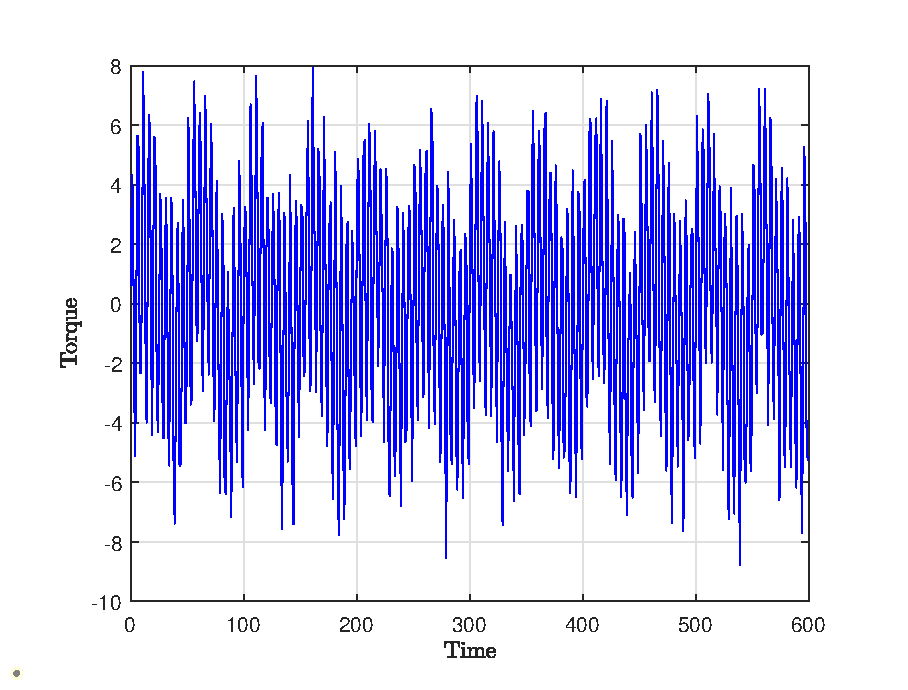
\includegraphics[width=250pt]{chapters/ch-fuzzy-control-system/figures/exp_vibration_detection_signal.eps}
	\caption{Measured torque.}
	\label{ch:fcs:fig:exp_vibration_detection_signal}
\end{figure}

\begin{figure}
	\centering
	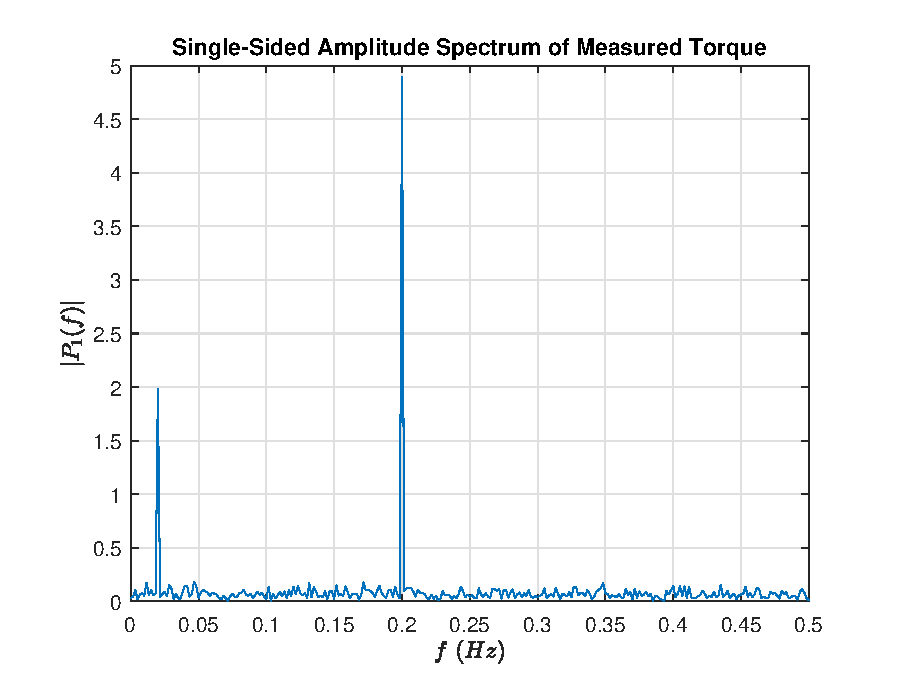
\includegraphics[width=250pt]{chapters/ch-fuzzy-control-system/figures/exp_vibration_detection_signal_fft.eps}
	\caption{Measured torque single-sided amplitude spectrum.}
	\label{ch:fcs:fig:exp_vibration_detection_signal_fft}
\end{figure}

If increase the frequency from $0.2Hz$ to $0.45Hz$, i.e., let 
\begin{lstlisting}
measured_torque = 5*sin(2*pi*0.4*t);
measured_torque = measured_torque + 2*sin(2*pi*0.02*t);
measured_torque = measured_torque + normrnd(0, 1, [1, length(measured_torque)]);
\end{lstlisting}
the likelihood becomes $0.60$. If further drop the amplitude and let
\begin{lstlisting}
measured_torque = 2*sin(2*pi*0.4*t);
measured_torque = measured_torque + 1*sin(2*pi*0.02*t);
measured_torque = measured_torque + normrnd(0, 1, [1, length(measured_torque)]);
\end{lstlisting}
the likelihood further drops to $0.30$. By an exhaustive search, we can plot likelihood as a function of oscillation frequency and amplitude as given in Fig. XXX.

\begin{figure}
	\centering
	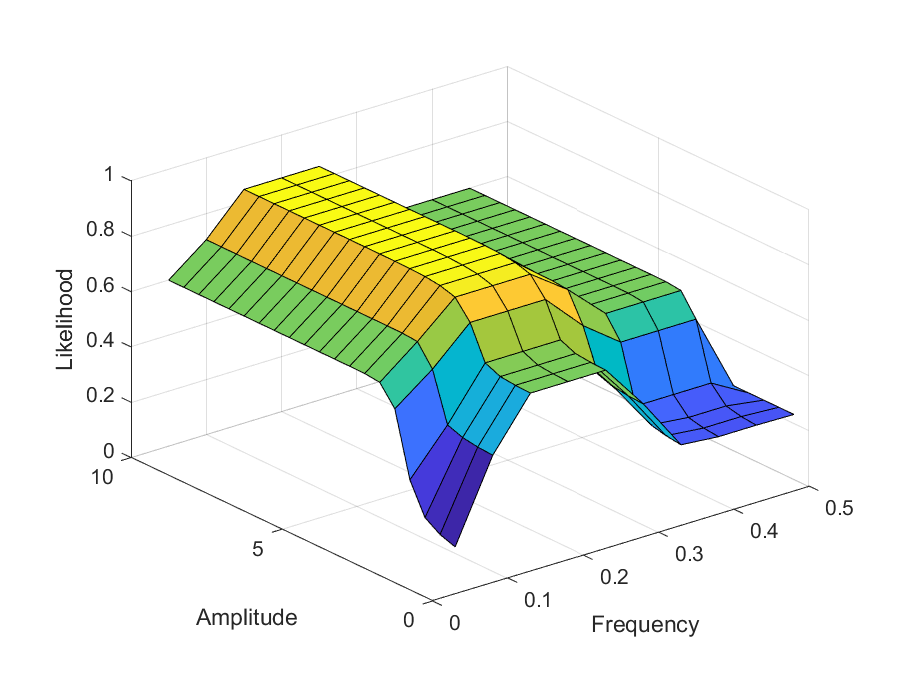
\includegraphics[width=250pt]{chapters/ch-fuzzy-control-system/figures/exp_vibration_detection_gensurf1.eps}
	\caption{Likelihood of vibration as a function of oscillation frequency and amplitude.}
	\label{ch:fcs:fig:exp_vibration_detection_gensurf1}
\end{figure}

Consider programming using MATLAB built-in tools to reproduce the above results. MATLAB provides variety choice of fuzzy inference systems. In this example, \verb|mamfis| is used as follows.
\begin{lstlisting}
vd_fis = mamfis( ...
	'NumInputs', 2, ...
	'NumInputMFs', [3, 2], ...
	'NumOutputs', 1, ...
	'NumOutputMFs', 4, ...
	'AddRule', 'none' ...
	);
% ios
vd_fis.Inputs(1).Name = 'torque_frequency';
vd_fis.Inputs(1).Range = [0, 0.5];
vd_fis.Inputs(1).MembershipFunctions(1).Name = 'low';
vd_fis.Inputs(1).MembershipFunctions(1).Type = 'trapmf';
vd_fis.Inputs(1).MembershipFunctions(1).Parameters = [-1, 0, 0.05, 0.15];
vd_fis.Inputs(1).MembershipFunctions(2).Name = 'fine';
vd_fis.Inputs(1).MembershipFunctions(2).Type = 'trapmf';
vd_fis.Inputs(1).MembershipFunctions(2).Parameters = [0.05, 0.15, 0.25, 0.35];
vd_fis.Inputs(1).MembershipFunctions(3).Name = 'high';
vd_fis.Inputs(1).MembershipFunctions(3).Type = 'trapmf';
vd_fis.Inputs(1).MembershipFunctions(3).Parameters = [0.25, 0.40, 0.5, 1];
vd_fis.Inputs(2).Name = 'torque_amplitude';
vd_fis.Inputs(2).Range = [0, 10];
vd_fis.Inputs(2).MembershipFunctions(1).Name = 'low';
vd_fis.Inputs(2).MembershipFunctions(1).Type = 'gbellmf';
vd_fis.Inputs(2).MembershipFunctions(1).Parameters = [4, 10, -2];
vd_fis.Inputs(2).MembershipFunctions(2).Name = 'fine';
vd_fis.Inputs(2).MembershipFunctions(2).Type = 'gbellmf';
vd_fis.Inputs(2).MembershipFunctions(2).Parameters = [5, 5, 8];
plotmf(vd_fis, 'input', 1, 1000)
vd_fis.Outputs(1).Name = 'vibration_likelihood';
vd_fis.Outputs(1).Range = [0, 1];
vd_fis.Outputs(1).MembershipFunctions(1).Name = 'very_unlikely';
vd_fis.Outputs(1).MembershipFunctions(1).Type = 'gbellmf';
vd_fis.Outputs(1).MembershipFunctions(1).Parameters = [0.2, 5, 0];
vd_fis.Outputs(1).MembershipFunctions(2).Name = 'unlikely';
vd_fis.Outputs(1).MembershipFunctions(2).Type = 'gbellmf';
vd_fis.Outputs(1).MembershipFunctions(2).Parameters = [0.15, 3, 0.3];
vd_fis.Outputs(1).MembershipFunctions(3).Name = 'likely';
vd_fis.Outputs(1).MembershipFunctions(3).Type = 'gbellmf';
vd_fis.Outputs(1).MembershipFunctions(3).Parameters = [0.15, 3, 0.6];
vd_fis.Outputs(1).MembershipFunctions(4).Name = 'very_likely';
vd_fis.Outputs(1).MembershipFunctions(4).Type = 'gbellmf';
vd_fis.Outputs(1).MembershipFunctions(4).Parameters = [0.3, 5, 1];
plotmf(vd_fis, 'output', 1, 1000)
% rules
rules = ["if torque_frequency is fine and torque_amplitude is fine then vibration_likelihood is very_likely"; ...
	"if torque_frequency is fine and torque_amplitude is low then vibration_likelihood is likely"; ...
	"if torque_frequency is high and torque_amplitude is fine then vibration_likelihood is likely"; ...
	"if torque_frequency is high and torque_amplitude is low then vibration_likelihood is unlikely"; ...
	"if torque_frequency is low and torque_amplitude is fine then vibration_likelihood is likely"; ...
	"if torque_frequency is low and torque_amplitude is low then vibration_likelihood is very_unlikely"; ...
	"if torque_amplitude is fine then vibration_likelihood is likely" ...
	];
vd_fis = addRule(vd_fis, rules);
\end{lstlisting}

Use
\begin{lstlisting}
	evalfis(vd_fis, [<frequency>, <amplitude>])
\end{lstlisting}
to get the output of the fuzzy controller. Use
\begin{lstlisting}
	gensurf(vd_fis)
\end{lstlisting}
to obtain the plot of likelihood as a function of the oscillation frequency and amplitude as given in Fig. \ref{ch:fcs:fig:exp_vibration_detection_gensurf2}, which is similar with Fig. \ref{ch:fcs:fig:exp_vibration_detection_gensurf1}.

\begin{figure}
	\centering
	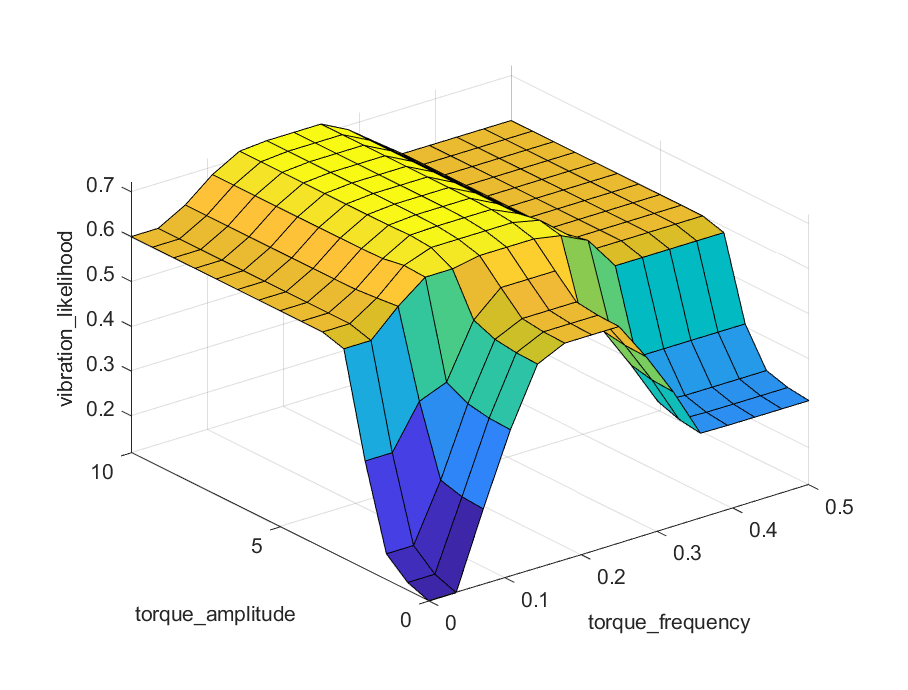
\includegraphics[width=250pt]{chapters/ch-fuzzy-control-system/figures/exp_vibration_detection_gensurf2.eps}
	\caption{Likelihood of vibration as a function of oscillation frequency and amplitude using \texttt{mamfis}.}
	\label{ch:fcs:fig:exp_vibration_detection_gensurf2}
\end{figure}



